\documentclass[11pt]{article}
\usepackage[romanian]{babel}
\usepackage[utf8]{inputenc}
\usepackage[T1]{fontenc}
\usepackage{amsmath}
\usepackage{amsfonts}
\usepackage{amssymb}
\usepackage[version=4]{mhchem}
\usepackage{stmaryrd}
\usepackage{graphicx}
\usepackage[export]{adjustbox}
\graphicspath{ {./images/} }

\begin{document}
Private Equity Funds of Funds Investment

\section*{Four Benefits to Investing in PE Fund of Funds}
There are several advantages to investing in PE FoFs:

\begin{enumerate}
  \item Diversification benefits. PE FoFs invest across PE funds and vintage years. This has the effect of reducing performance dispersion compared to investing in a single PE fund. In addition, it also lowers downside risk when compared to investing in a single PE fund. Weidig and Mathonet (2004) gave the example that for venture capital, the probability of a total loss of capital invested is around $30 \%$ for direct investments and close to zero for funds and funds of funds. The probability of a loss for a fund is around $30 \%$, but small for a fund of funds.

  \item Professional Management. The manager of a PE FoF has a dedicated investment team with experience in identifying top-performing PE funds. They are likely to have a network in the PE space that they are targeting, either through staff with experience working in PE funds, or personal networks developed over time. This helps them identify GPs and conduct reference checks. Lastly, FoFs invest in funds on a large scale, giving them economies of scale that are not available to smaller investors, and they typically have a long-term horizon and targeted pool of capital.

  \item Access to funds, specific strategy, or geography. Many of the PE FoFs are specialized funds focusing on a particular strategy, such as venture capital, growth equity, or middle market buyouts. They could also focus on a specific geography such as Europe or Asia. The expertise and domain knowledge of the manager is difficult to replicate by smaller LPs without the help of external advisors. Importantly, some of the FoFs may have established relationships with leading venture capital firms that are heavily sought after. These FoFs may be able to provide investors access to these leading venture capital firms.

  \item Lower capital commitment. The minimum investment for a single PE fund may be $\$ 1 \mathrm{~m},{ }^{1}$ Using data from Preqin from 2015 to 2020 , the median minimum investment requirement for venture capital and buyout funds, as well as funds of funds, was $\$ 1$ million. thus an investor may need a large amount of capital to create a portfolio of PE funds. In comparison, the minimum investment for PE FoFs may be lower and the investor can obtain the diversification without a large capital commitment. Also, some investors may not meet the minimum investment requirement for PE funds. But by investing through PE FoFs, they enjoy the economies of scale and may gain access to PE funds that they otherwise would be unable to.

\end{enumerate}

\section*{Four Disadvantages in Investing in PE Fund of Funds}
The following are some disadvantages to investing in PE FoFs:

\begin{enumerate}
  \item Additional layer of fees. PE FoFs charge management fee and carried interest in addition to the layer of the fees charged by the underlying PE funds. The management fee is typically $0.5 \%$ to $1.0 \%$ of committed capital with carried interest of $5 \%$ to $10 \%$ of realized gains, which will reduce the returns the investor would have earned by directly investing in the portfolio of PE funds. For large institutional LPs who have the experience, the bargaining power, and the access to PE funds, the fund selection and risk reduction benefits of a PE FoFs is significantly reduced. However, for smaller institutional LPs, they may find that the cost of investing in a PE FoF is lower than if they had built an internal team to identify and monitor a portfolio of PE managers.

  \item GP relationship remains with the manager of the PE FoF. The manager of the PE FoF has direct relationships with the underlying GPs as she is sourcing and evaluating the managers in her portfolio. Investors of a PE FoFs do not have direct access to the underlying fund managers without an introduction from manager of the PE FoF.

  \item Less transparency. Since PE FoFs are investing across funds, the information on underlying portfolio companies will be limited. Investors in PE funds may be able to obtain more detailed information on the portfolio companies held in the underlying funds.

  \item Lack of liquidity. The typical PE fund has a fund life of 7 to 10 years. PE FoFs, or primary FoFs, may have longer fund life than the typical PE funds because they are investing in the PE funds across vintage years. In contrast, secondary FoFs may have shorter fund lives than primary FoFs. The majority of PE FoFs are closed-ended with finite fund life. This matches the underlying PE funds, which are likely to be closed-ended as well. On the other hand, there are some openended PE FoFs. They are likely to have redemption features to provide limited liquidity on a quarterly or monthly basis. But the redemption features may come at a cost in the form or redemption penalty, or the cash drag on returns as the FoF hold cash balance to meet redemptions. In addition, most open-ended funds would have some gating mechanism such as a cap on the total redemption to protect the fund. Thus the liquidity from open-ended fund will be limited in times of market turmoil. Secondary market for PE FoFs stake may not be active, which makes exiting before the end of fund life challenging.

\end{enumerate}

\section*{Factors Driving the PE Fund of Funds Market}
The market for PE FoFs has changed significantly over the last decade. At first glance, it looked like fundraising had peaked in 2007-08 in the exhibit Global PE FoF Fundraising Activity, while the overall private equity industry has grown substantially over the last decade. On closer examination, the business models of PE FoFs have been evolving. The GPs of many FoFs have expanded their offerings to include secondaries, co-investments, and separate accounts as the sophistication of investors has increased. Despite the changing conditions, the value proposition of PE FoFs to investors remains relevant.

\begin{center}
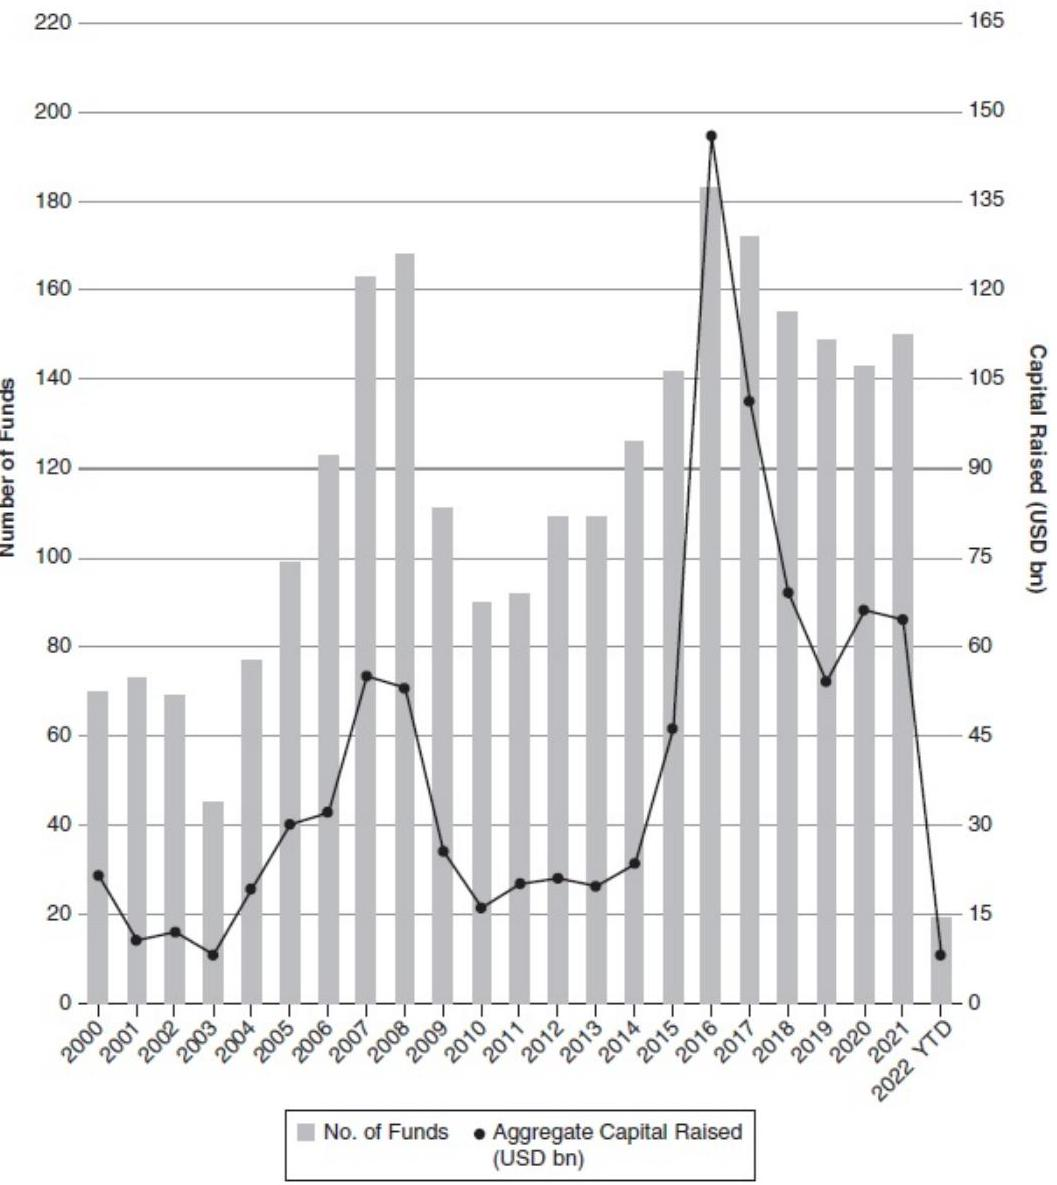
\includegraphics[max width=\textwidth]{2024_04_10_558733fce4b45c386018g-3}
\end{center}

Global PE FoF Fundraising Activity

Source: Preqin, 2022

Easy way to access PE. PE FoFs are a good way for new investors to obtain their initial exposure to the asset class. The structure of PE FoFs creates an easy way to access private equity for investors who may lack the knowledge or resources to do so. For many investors, FoFs remain a springboard for a PE program. It offers significant diversification and alleviates many of the constraints faced by investors.

Smaller PE program. If an investor's portfolio base is not large, they may not have enough capital to build a diversified portfolio of PE funds. An investment in PE FoF may be a good way to access the PE asset class.

Complement to existing PE Program. A PE FoF program can complement existing PE program. For example, a FoF could offer access to a venture capital fund that may not exist in the program. While a European investor may be comfortable investing directly in European PE funds, they may delegate the manager selection and due diligence process to a FoF manager in order to access private equity opportunities in the US or Asian markets.

Increased complexity of PE operational due diligence. As LPs have become increasingly focused on operational risk in PE funds, PE GPs have increasingly enhanced the complexity and strength of their operations. This increase in operational complexity has also been driven by growing complexity in regard to the regulatory compliance obligations of PE firms. As such, a PE FoF can assist many LPs who do not have the requisite expertise in performing operational due diligence (ODD) on PE funds in order to better vet these operational and compliance risks at PE firms.


\end{document}